\chapter{Requirements Analysis}%
\label{chapter:requirementsAnalysis}

\begin{introduction}
This chapter defines the specification of the proposed system, combining insights from meetings with Lightmobie, \ac{emel}, and the literature. It begins with the requirements, organized by the FURPS model and extended with functional and system constraints. Then, the use cases and workflow are presented to illustrate how each role interacts with the system and how information flows during maintenance. Finally, a set of statuses is introduced to track the progress of each service request, ensuring transparency and consistency throughout the process.
\end{introduction} 




\section{Application Requirements}
The requirements for the application were defined based on insights gathered from multiple sources. These include meetings with stakeholders from Lightmobie and \ac{emel}, as well as findings from the literature review. To structure and classify these requirements, the FURPS model was adopted, which organizes them into functional and non-functional categories. ~\cite{furps, furps2} 

\subsection{Functional Requirements and Use cases}
The functional requirements define the operations and features that the system must provide to support the daily activities of its users. These requirements were complemented by the creation of a set of \textbf{use cases} that illustrate how users interact with the system to accomplish specific goals. This approach helps capture requirements from the user’s perspective, ensuring that the solution aligns closely with real operational workflows.

The application supports multiple user roles, each responsible for distinct aspects of the maintenance process: administrator, receptionist, mechanic, warehouse manager, workshop manager, and client. In addition, an administrator view provides global oversight and configuration capabilities to ensure the system operates efficiently across all dealerships.


\subsubsection{Administrator}

The administrator is responsible for configuring the system and managing essential data that supports dealership operations. This includes maintaining records of dealerships, employees, and vehicle parts, as well as defining the types of maintenance tasks that can be performed. Through these actions, the administrator ensures that the system's structure remains consistent and up to date.


\begin{itemize}
    \item Create, edit, view, and remove task types
    \item Manage dealerships (create, edit, view, remove, add/remove vehicle types)
    \item Manage vehicle parts (create, edit, view, remove)
    \item Create and view dealership employees
\end{itemize}

\subsubsection{Receptionist}

The receptionist acts as the main point of contact between the client and the workshop. This role involves registering vehicles, creating and updating maintenance requests, and keeping clients informed about the progress of their services. 

\begin{itemize}
    \item Switch interface language between English and Portuguese
    \item View daily working hours and user-specific hours
    \item Schedule vehicle reception (registration number, client email, owner name, reception date)
    \item Create maintenance (expected budget, tasks, expected conclusion date)
    \item View active maintenances (client name, registration number, entity, creation date, evaluation date, expected conclusion date, budget, planned work hours, tasks)
    \item Receive notifications on budget or deadline changes in maintenance
    \item Confirm or reject maintenance changes
    \item Cancel maintenance
    \item Conclude maintenance
    \item Notify when all maintenance tasks are completed
\end{itemize}

To model these interactions, several use cases were defined to describe the receptionist's typical activities and system interactions.


\begin{itemize}
    \item \textbf{Use Case 1.1 – Maintenance Schedule}\\
    \textit{Scenario:} Client arrives with a vehicle for repair.\\
    \textit{Objective:} Create a new maintenance request.\\
    \textit{System:} Receptionist enters vehicle and client details, evaluation date, entity, client notes, and requested tasks.
    \item \textbf{Use Case 1.2 – Maintenance Approval}\\
    \textit{Scenario:} Vehicle evaluation concludes.\\
    \textit{Objective:} Set budget, completion date, and tasks.\\
    \textit{System:} Receptionist receives evaluation notification, consults customer, system calculates price, completion date set.
    \item \textbf{Use Case 1.3 – Collect Maintenance Information}\\
    \textit{Scenario:} Client contacts dealership for maintenance status.\\
    \textit{Objective:} View details of a maintenance request.\\
    \textit{System:} Receptionist searches by vehicle or client and views relevant details.
    \item \textbf{Use Case 1.4 – Accept Maintenance Changes}\\
    \textit{Scenario:} Issue arises and client accepts proposed changes.\\
    \textit{Objective:} Accept changes to maintenance.\\
    \textit{System:} Receptionist navigates to maintenance changes section on maintenance details and approves modifications.
    \item \textbf{Use Case 1.5 – Refuse Maintenance Changes}\\
    \textit{Scenario:} Issue arises and client refuses the change.\\
    \textit{Objective:} Refuse changes to maintenance.\\
    \textit{System:} Receptionist navigates to maintenance changes section on maintenance details and rejects the modification.
    \item \textbf{Use Case 1.6 – Vehicle Delivery}\\
    \textit{Scenario:} Vehicle is ready to be delivered to the client.\\
    \textit{Objective:} Complete maintenance process.\\
    \textit{System:} Maintenance marked as concluded and the delivery date is registered.
    \item \textbf{Use Case 1.7 – Cancel Maintenance}\\
    \textit{Scenario:} Client rejects agreement and retrieves vehicle.\\
    \textit{Objective:} Cancel the maintenance.\\
    \textit{System:} Receptionist cancels maintenance within details section and invalidates all uncompleted tasks.
    \item \textbf{Use Case 1.8 – Cancel Task}\\
    \textit{Scenario:} Issue leads to cancellation of a specific task.\\
    \textit{Objective:} Cancel problematic task.\\
    \textit{System:} Receptionist cancels task in maintenance changes section.
\end{itemize}


\subsubsection{Mechanic}

Mechanics are responsible for performing the actual maintenance work, including diagnostics, repairs, and part replacements. Their \ac{UI} provides clear visibility into assigned tasks, progress tracking, and reporting tools to ensure maintenance quality and accountability. Mechanics can pause, resume, and complete tasks while adding comments or observations about the performed work.


\begin{itemize}
    \item Switch interface language between English and Portuguese
    \item View today's tasks
    \item Pause and continue tasks (e.g., for breaks)
    \item View maintenance task details (registration number, task type, parts, step descriptions, needed parts, client desired tasks)
    \item Finalize a task and comment before completion
    \item View evaluation tasks (maintenance tasks needed, client comment)
    \item If evaluations are not used, maintenance concludes when a mechanic finishes the evaluation task
\end{itemize}

The following use cases illustrate the main interactions of the mechanic with the system during daily operations:

\begin{itemize}
    \item \textbf{Use Case 2.1 – View To-Do List}\\
    \textit{Scenario:} Mechanic begins shift.\\
    \textit{Objective:} View tasks for completion.\\
    \textit{System:} System presents assigned and available tasks with details.
    \item \textbf{Use Case 2.2 – Conduct Vehicle Analysis}\\
    \textit{Scenario:} Vehicle needs analysis.\\
    \textit{Objective:} Confirm initial assessment and detect additional issues.\\
    \textit{System:} Mechanic reviews and selects analysis tasks.
    \item \textbf{Use Case 2.3 – Complete maintenance}\\
    \textit{Scenario:} Maintenance tasks completed.\\
    \textit{Objective:} Mark tasks as finished.\\
    \textit{System:} Mechanic logs finished tasks for vehicle.
    \item \textbf{Use Case 2.4 – Execute Maintenance Task}\\
    \textit{Scenario:} Vehicle scheduled for specific maintenance.\\
    \textit{Objective:} Complete task following required steps.\\
    \textit{System:} System presents a stepwise guidance.
    \item \textbf{Use Case 2.5 – Change Task}\\
    \textit{Scenario:} Task has incorrect part associated.\\
    \textit{Objective:} Rectify the incorrect task.\\
    \textit{System:} Mechanic submits a task change request for client approval if the budget is impacted.
    \item \textbf{Use Case 2.6 – Continue Task}\\
    \textit{Scenario:} Task was paused.\\
    \textit{Objective:} Resume incomplete task.\\
    \textit{System:} Mechanic selects task to continue from the list.
\end{itemize}


\subsubsection{Warehouse Manager}

Warehouse managers oversee all operations related to parts and inventory control. Their responsibilities include managing stock levels, registering purchases, and maintaining supplier information to ensure the workshop has all necessary materials for ongoing maintenance work. The system provides real-time visibility of part availability and supports efficient purchase workflows.


\begin{itemize}
    \item Switch interface language between English and Portuguese
    \item View dealership inventory (name, code, quantity, warehouse location, description, category, price, quantity per group, min/max values for alarms/purchase requests)
    \item Edit part type details (location, min/max values, purchase request quantities)
    \item View quantity changes over time for each part
    \item See supplier details (name, phone, email, address, contract parts with start/end date)
    \item Create purchase requests (motive, parts, quantity per part)
    \item View all purchases (status, arrival date, total price, motive, creation date, parts, stock quantity, price, associated tasks)
    \item Register expected arrival date or delays for purchases
    \item Finalize delivery purchase by registering received parts
\end{itemize}

The following use cases describe the typical operations of the warehouse manager within the system:


\begin{itemize}
    \item \textbf{Use Case 3.1 – View Stock}\\
    \textit{Scenario:} Need to check part quantities.\\
    \textit{Objective:} Show inventory levels.\\
    \textit{System:} List all parts with current quantities.
    \item \textbf{Use Case 3.2 – Request Purchase}\\
    \textit{Scenario:} Low stock identified.\\
    \textit{Objective:} Request authorization to purchase.\\
    \textit{System:} Place purchase order, notify administrator for approval.
    \item \textbf{Use Case 3.3 – Register Purchase}\\
    \textit{Scenario:} Purchase request approved.\\
    \textit{Objective:} Order new parts from the supplier.\\
    \textit{System:} Operator enters the expected arrival date of the parts.
    \item \textbf{Use Case 3.4 – Register New Parts}\\
    \textit{Scenario:} Parts arrive from supplier.\\
    \textit{Objective:} Add new stock to inventory.\\
    \textit{System:} Operator updates parts quantity and purchase completion date.
    \item \textbf{Use Case 3.5 – Edit Inventory}\\
    \textit{Scenario:} Need to alter inventory details.\\
    \textit{Objective:} Update inventory information.\\
    \textit{System:} Changes made to part location, code or purchase generation.
    \item \textbf{Use Case 3.6 – Create Purchase Delay}\\
    \textit{Scenario:} Purchase is delayed.\\
    \textit{Objective:} Update expected arrival.\\
    \textit{System:} Operator enters revised arrival date.
\end{itemize}




\subsubsection{Workshop Manager}

The workshop manager supervises the overall maintenance process, ensuring efficient task allocation, quality control, and resource management. This role bridges the communication between operational and administrative levels, authorizing purchases, monitoring statistics, and managing both employees and partnerships with external entities.


\begin{itemize}
    \item Switch interface language between English and Portuguese
    \item View daily and user-specific working hours
    \item View unassigned tasks
    \item Assign tasks to mechanics
    \item View and manage active maintenances (full details including done/planned tasks)
    \item Add tasks to active maintenances
    \item View completed tasks with filters (client, vehicle, date), details (client name, vehicle registration, entity, creation date, evaluation date, conclusion date, budget, hours, price), and export as PDF
    \item View monthly maintenance revenue and total hours worked
    \item Assign purchases to operators
    \item View purchase requests (price, motive, creation date, parts info)
    \item Authorize or reject purchase requests
    \item Create supplier records (name, phone, email, address, contract parts/details)
    \item View suppliers and partnerships with bike sharing entities; accept/reject partnerships
    \item View employee list (email, name, DOB, phone, sex, role); create employee records (all listed data plus password)
\end{itemize}

The following use cases summarize the key activities of the workshop manager:

\begin{itemize}
    \item \textbf{Use Case 4.1 – Assign Tasks}\\
    \textit{Scenario:} New maintenance requested.\\
    \textit{Objective:} Distribute tasks among staff.\\
    \textit{System:} Manager assigns tasks to employees.
    \item \textbf{Use Case 4.2 – Authorize Purchase}\\
    \textit{Scenario:} Purchase request received.\\
    \textit{Objective:} Accept/reject authorization.\\
    \textit{System:} Manager approves or rejects the request.
    \item \textbf{Use Case 4.3 – View Maintenance History}\\
    \textit{Scenario:} Access history of performed maintenance.\\
    \textit{Objective:} Review details.\\
    \textit{System:} Historical maintenance and detail review.
    \item \textbf{Use Case 4.4 – Compile Statistics}\\
    \textit{Scenario:} Manager wants maintenance statistics.\\
    \textit{Objective:} Present graphical summaries.\\
    \textit{System:} System generates graphs of parts replaced, purchase volumes, costs, and ratings.
    \item \textbf{Use Case 4.5 – Assign Roles}\\
    \textit{Scenario:} New employee hired.\\
    \textit{Objective:} Set role and permissions.\\
    \textit{System:} Assignment in employee record.
    \item \textbf{Use Case 4.6 – Add New Task}\\
    \textit{Scenario:} Ongoing maintenance lacks a task.\\
    \textit{Objective:} Add required task after client validation.\\
    \textit{System:} Manager adds task to maintenance, client validates addition.
    \item \textbf{Use Case 4.7 – Create Employee}\\
    \textit{Scenario:} Hiring new workshop staff.\\
    \textit{Objective:} Register new employee.\\
    \textit{System:} Manager completes employee registration in system.
    \item \textbf{Use Case 4.8 – Partnership Decision}\\
    \textit{Scenario:} Entity proposes partnership.\\
    \textit{Objective:} Accept or reject partnership.\\
    \textit{System:} Status of partnership request updated by manager.
\end{itemize}




\subsubsection{Client}

Clients interact with the system through a \ac{UI} that allows them to stay informed about their vehicle’s maintenance process. They can review progress, receive notifications when maintenance is completed, and provide feedback on service quality. This promotes transparency and strengthens trust between clients and workshops.


\begin{itemize}
    \item View active maintenance information
    \item View maintenance history
    \item evaluate the perception of the service quality 
    \item evaluate the expected service quality 
\end{itemize}

The following use cases capture typical client interactions within the platform:

\begin{itemize}
    \item \textbf{Use Case 5.1 – View Maintenance Status}\\
    \textit{Scenario:} Client checks current status.\\
    \textit{Objective:} Display maintenance progress.\\
    \textit{System:} System displays completed and pending steps.
    \item \textbf{Use Case 5.2 – Receive End Notification}\\
    \textit{Scenario:} Maintenance completed.\\
    \textit{Objective:} Notify client.\\
    \textit{System:} email sent.
    \item \textbf{Use Case 5.3 – Rate Completed Service}\\
    \textit{Scenario:} Maintenance concludes and client retrieves vehicle.\\
    \textit{Objective:} Obtain service feedback.\\
    \textit{System:} Rating form offered in app.
    \item \textbf{Use Case 5.4 – Rate Expected Service}\\
    \textit{Scenario:} Maintenance agreement finalized.\\
    \textit{Objective:} Gather rating on expected service.\\
    \textit{System:} Rating form presented to client.
    \item \textbf{Use Case 5.5 – View Maintenance History}\\
    \textit{Scenario:} Client reviews previous maintenances.\\
    \textit{Objective:} Show maintenance history.\\
    \textit{System:} History shown and accessible via app interface.
\end{itemize}


\subsubsection{System Requirements}

The system also enforces several logical and structural requirements to ensure consistency, integrity, and operational efficiency, as summarized below:

\begin{itemize}
    \item The system must generate a repair report for each maintenance completed.
    \item Each maintenance task must have a defined sequence to ensure correct order of execution.
    \item Each purchase record may include multiple parts, along with their respective details.
    \item The system must generate a purchase request when an available quantity of a part is under a determined threshold. 
    \item Dealerships can only create maintenance tasks for vehicles belonging to their \acs{PBS} partners; otherwise, they may only accept maintenance from independent clients.
    \item The workflow must be flexible enough to support both general vehicle maintenance processes and the specific procedures used by \ac{emel}.
\end{itemize}

% \section{Application Use Cases}
% To capture how different users interact with the system, a set of use cases was defined. The following subsections present the use cases for each user type, outlining their primary responsibilities and the actions they can perform within the application.


\subsection{Non-Functional Requirements}

The non-functional requirements of the system were defined following the FURPS model and are summarized in Table~\ref{table:non_functional_requirements}. These requirements ensure that, \textbf{beyond providing the necessary functionalities}, the system also delivers \textbf{high standards of quality, performance, usability, and maintainability}.


\begin{table}[htbp]
\centering
\begin{tabular}{|l|p{10cm}|}
\hline
\textbf{Category} & \textbf{Requirement} \\ \hline
Scalability & The system must dynamically allocate resources to handle peak loads without service degradation. \\ \hline
Reliability & The system must ensure at least 99\% availability and be able to recover from failures within 4 hours. \\ \hline
Performance & The system should process at least 500 transactions per minute under normal conditions. \\ \hline
Usability & Training a new user to effectively use the system should take no longer than 8 hours. \\ \hline
Supportability & The system must be compatible with the latest versions of Chrome, Firefox, Microsoft Edge, and Safari. \\ \hline
\end{tabular} 
\caption{Non-Functional Requirements using FURPS Model}
\label{table:non_functional_requirements}
\end{table}



\section{Applications Workflow}

To provide a clear view of how users interact both with the system and with each other, a workflow diagram was created based on the defined use cases. The overall application workflow is presented in Figure~\ref{fig:appWorkflow}.

\begin{figure}[h]
  \caption{Use case flow chart of the Client, Receptionist, Mechanic, Warehouse Operator, and Workshop Manager.}
  \centering
  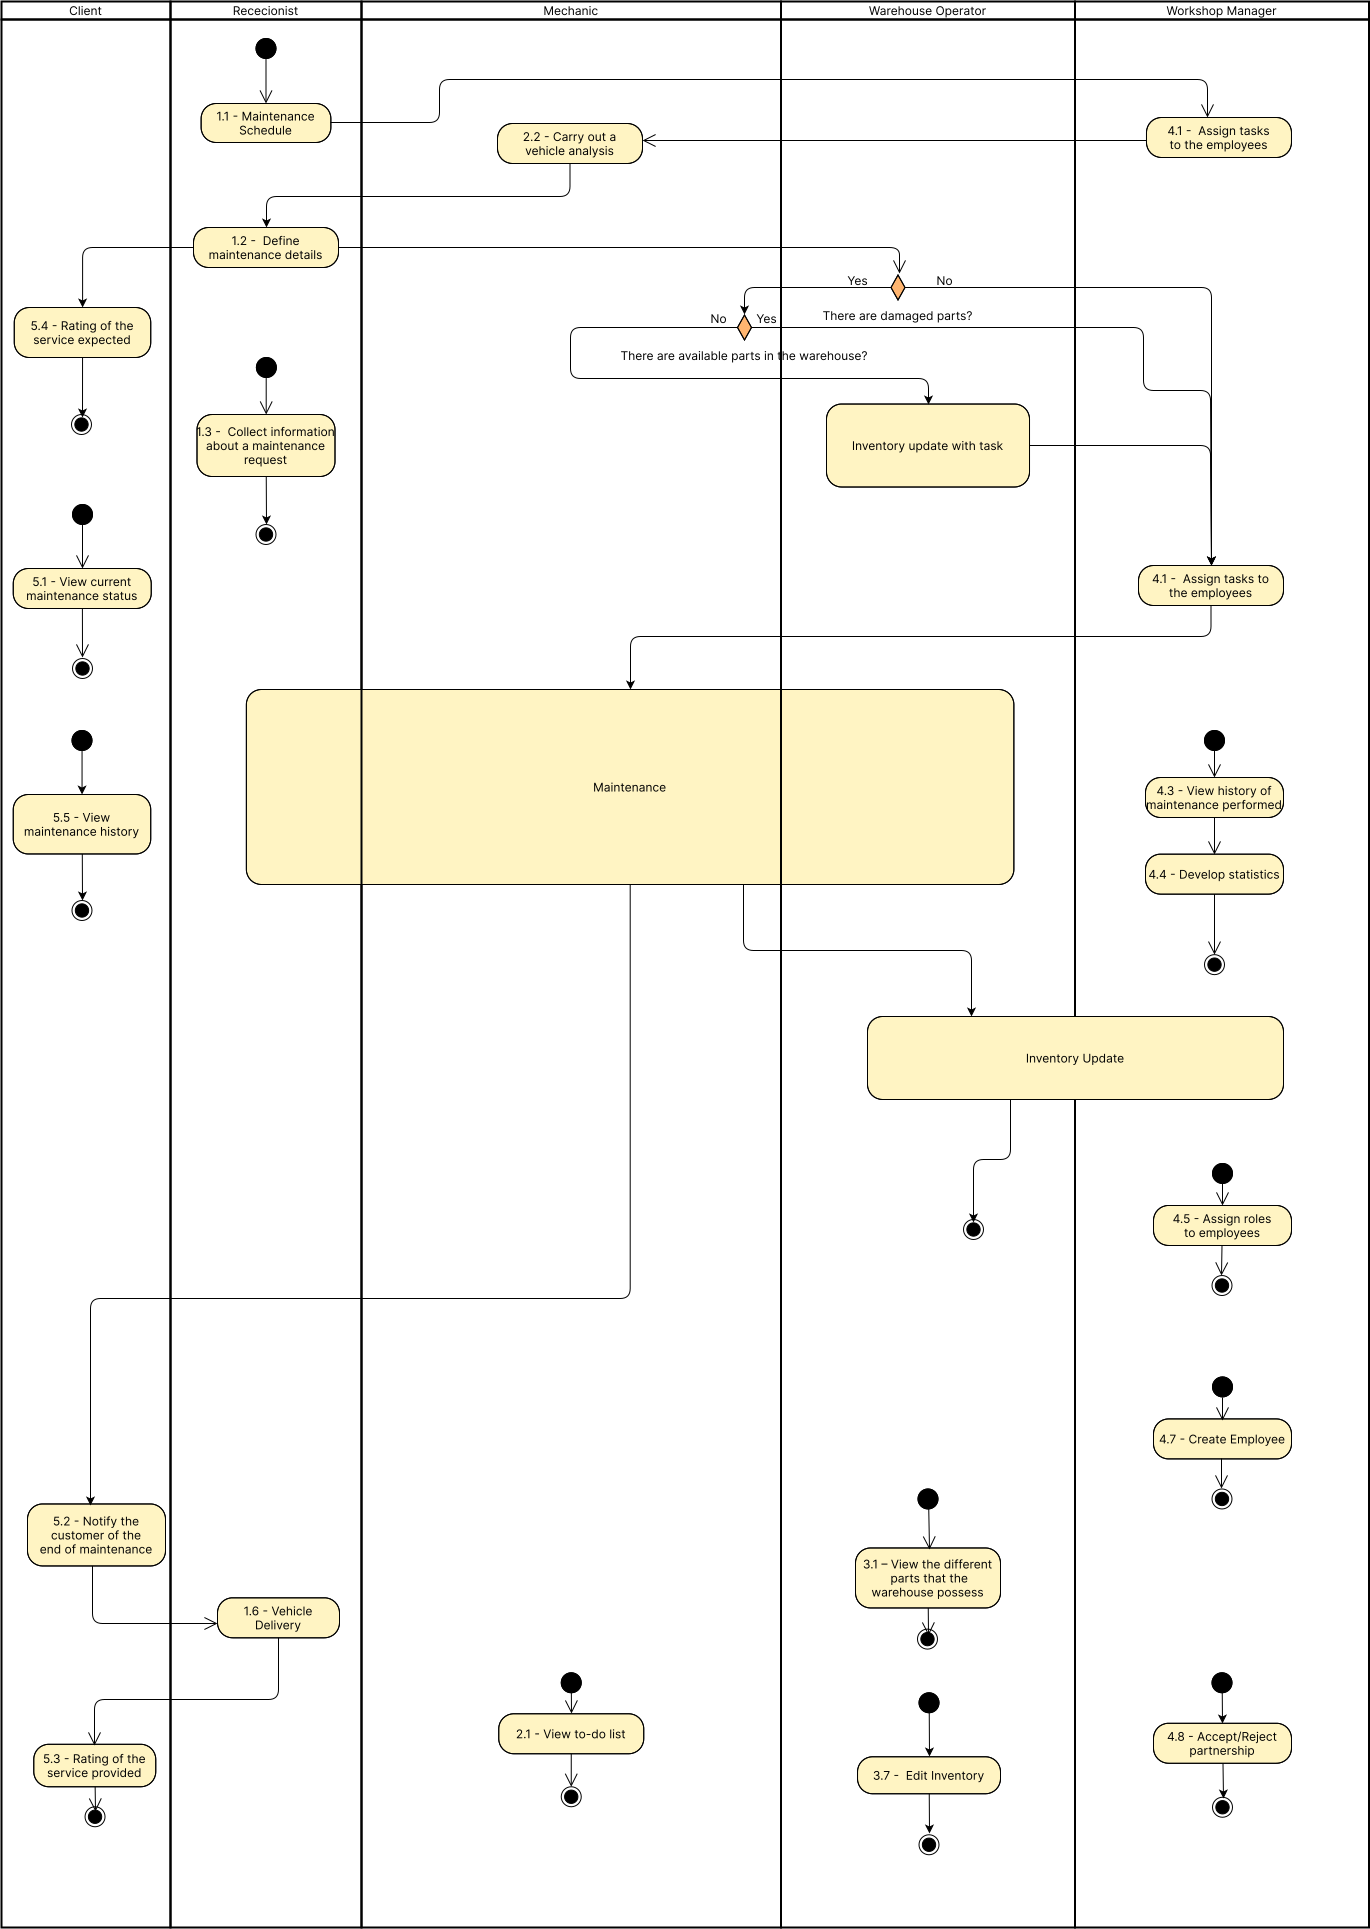
\includegraphics[width=\textwidth]{figs/UseCaseDiagram - General}
  \label{fig:appWorkflow}
\end{figure}

The main workflow begins when a client arrives at the dealership to request a vehicle maintenance. The receptionist records the request and registers this information in the system (Use Case 1.1). Once the request is created, a mechanic evaluates the vehicle, identifies problems, and specifies the necessary replacement parts (Use Case 2.2).

After this evaluation, the receptionist contacts the client to present the results. At this stage, both parties agree on the final maintenance plan, including the tasks to be performed, the expected delivery date, and the associated costs (Use Case 1.2). The client also provides an initial evaluation of the expected service quality on the client app (Use Case 5.4). When the plan is confirmed, the workshop manager receives a notification of the tasks and assigns them to the appropriate mechanics (Use Case 4.1).

From this point onward, the execution of the tasks may or may not require replacement parts. If no parts are needed, the mechanic performs the assigned maintenance (Use Case 2.6). If parts are required, the warehouse operator verifies stock availability. When the parts are available, they are delivered to the mechanic (Use Case 2.4). If they are not available, the operator submits a purchase request that must be approved by the workshop manager. If approved, the operator proceeds to order the parts (Use Case 3.3), register them in the system (Use Case 3.4), and deliver them to the mechanic. If the purchase request is rejected, the operator must restart the process with a new request (Use Case 3.2).

During the course of the maintenance, unexpected events may occur. A delivery delay (Use Case 3.6) or a task modification identified by the mechanic (Use Case 2.5) may affect the budget or the expected completion time. In such cases, the receptionist informs the client and requests a decision. The client may authorize the changes and allow the work to continue (Use Case 1.4), reject the changes while maintaining the original agreement (Use Case 1.5), refuse the changes but authorize the completion of the remaining approved tasks (Use Case 1.8), or cancel the maintenance entirely (Use Case 1.7). If the last option is chosen, all remaining tasks are invalidated, and the vehicle is prepared for check-out (Use Case 5.3).

When the maintenance tasks are completed, the system notifies the client that the vehicle is ready. The receptionist delivers the vehicle to the client (Use Case 1.6), after which the client is prompted by the application to rate the service (Use Cases 5.2 and 5.3).


\section{System Statuses} 

\subsection{Maintenance status} 

In order to ensure transparency and consistency during the maintenance process, it is important to track the overall progress of each service request through a set of predefined statuses. These statuses provide a structured view of the workflow, from the initial vehicle evaluation to its final delivery, while also capturing critical decision points that may alter the course of the process.

These are the \textit{maintenance status} key stages of this workflow:
\begin{itemize}
    \item \textbf{Wait Evaluation}: Inicial status when the vehicle is waiting to be inspected by the mechanic.
    \item \textbf{Wait Approval}: The mechanic has proposed tasks that require the client's approval.
    \item \textbf{During Maintenance}: Approved tasks are actively being executed by the workshop.
    \item \textbf{Maintenance Finished}: All tasks have either been completed or invalidated.
    \item \textbf{Delivered}: The vehicle is returned to the client after maintenance conclusion.
    \item \textbf{Canceled}: The client cancels the maintenance process mid-workflow.
\end{itemize}

\begin{figure}[h]
  \caption{Status flow chart of a maintenance workflow}
  \centering
  \includegraphics[width=\textwidth]{figs/Status/Maintenance/StatusDiagram}
  \label{fig:maintenanceFlowChart}
\end{figure}

The status transitions represented in Figure~\ref{fig:maintenanceFlowChart} outline how the workflow evolves over time:
\begin{itemize}
    \item \textbf{Wait Evaluation} $\rightarrow$ \textbf{Wait Approval}: After the mechanic completes the initial evaluation.
    \item \textbf{Wait Approval} $\rightarrow$ \textbf{During Maintenance}: Once the client approves the proposed tasks and budget.
    \item \textbf{During Maintenance} $\rightarrow$ \textbf{Maintenance Finished}: When all approved tasks are completed.
    \item \textbf{Maintenance Finished} $\rightarrow$ \textbf{Delivered}: The vehicle is handed back to the client.
    \item Any status $\rightarrow$ \textbf{Canceled}: If the client decides to cancel the maintenance process.
    \item \textbf{Wait Evaluation} $\rightarrow$ \textbf{Maintenance Finished}: If the dealership skips the evaluation step and the mechanic completes all tasks directly.
\end{itemize}

In Figure~\ref{fig:maintenanceUseCaseStatus} and ~\ref{fig:maintenanceDealershipUseCaseStatus} we can see how these status are divided in the use case flow of the application.

To further clarify how these statuses operate in practice, Figure~\ref{fig:maintenanceUseCaseStatus} and ~\ref{fig:maintenanceDealershipUseCaseStatus} illustrate their use within two different contexts: a dealership providing standard maintenance services and an entity managing maintenance without evaluation.


\begin{figure}[h]
  \caption{Use case flow chart of dealership maintenance, with statuses grouped by use cases}
  \centering
  \includegraphics[width=\textwidth]{figs/Status/Maintenance/UseCaseStatus}
  \label{fig:maintenanceUseCaseStatus}
\end{figure}


\begin{figure}[h]
  \caption{Use case flow chart of an entity managing maintenance without evaluation, with statuses grouped by use cases}
  \centering
  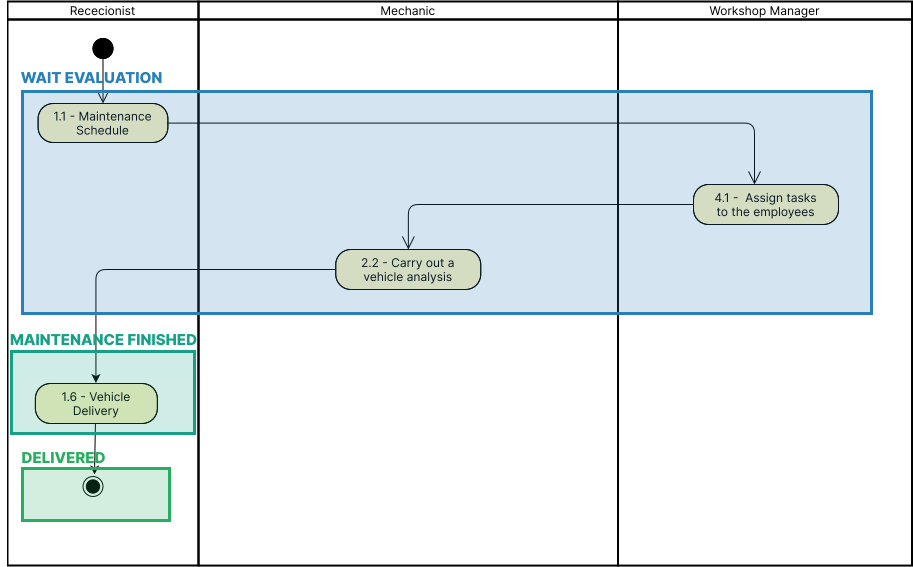
\includegraphics[width=\textwidth]{figs/Status/Maintenance/EntityDiagram}
  \label{fig:maintenanceDealershipUseCaseStatus}
\end{figure}


\subsection{Maintenance Change Status} 

During the course of maintenance, situations may arise that require modifications to the originally planned tasks or agreements. To manage this process effectively, the workflow is modeled through a set of statuses that capture the client's decision and define the subsequent path of action. 

\begin{itemize}
    \item \textbf{Ask Client}: Initial status when a maintenance change is identified and requires confirmation from the client.
    \item \textbf{Agreed}: The client accepts the proposed changes.
    \item \textbf{Refused}: The client rejects the changes, and the maintenance continues according to the previous agreement.
    \item \textbf{Task Canceled}: The client cancels the specific task that triggered the maintenance change.
    \item \textbf{Maintenance Canceled}: The client terminates the entire maintenance process.
\end{itemize}


\begin{figure}[h]
  \caption{Status flow chart of a maintenance change}
  \centering
  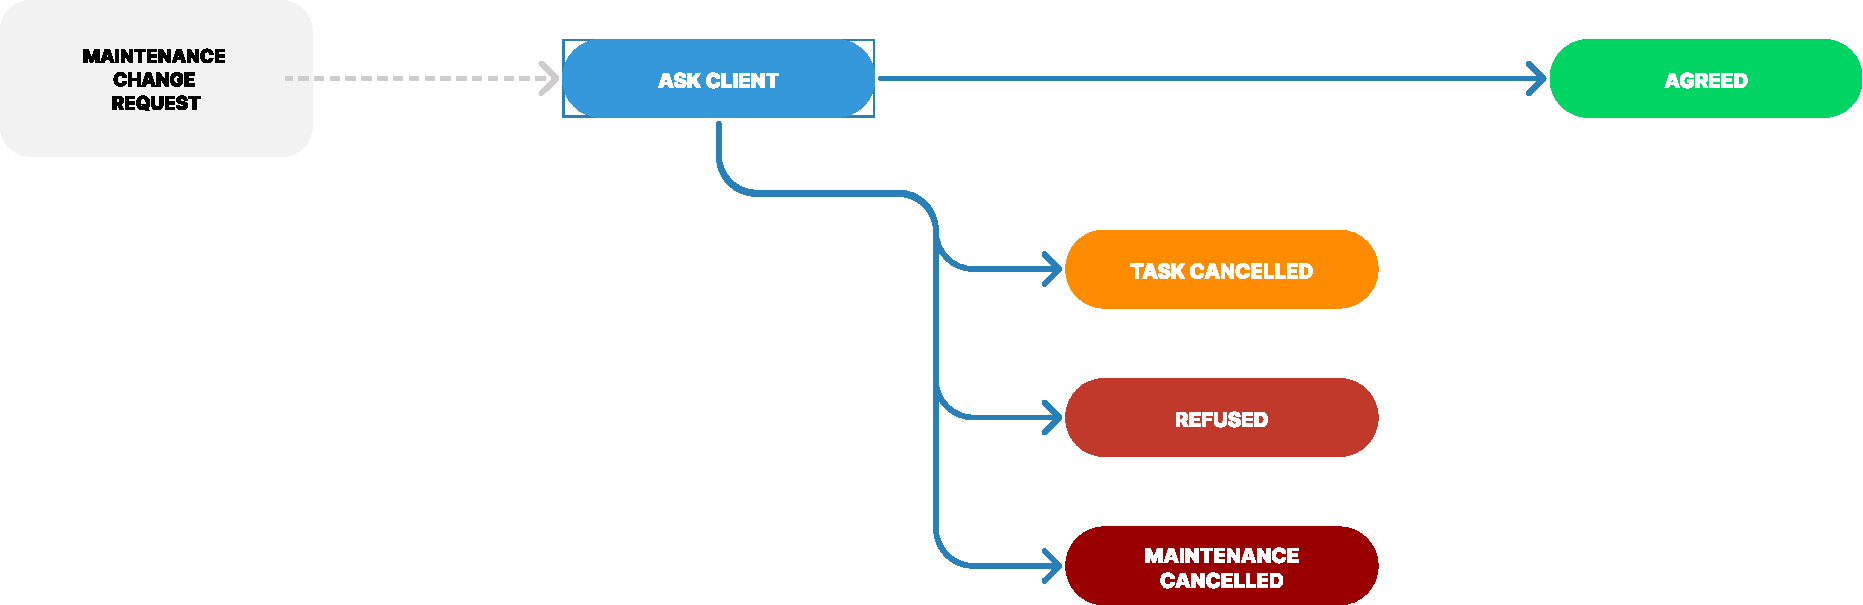
\includegraphics[width=\textwidth]{figs/Status/MaintenanceChange/StatusDiagram}
  \label{fig:maintenanceChangeFlowChart}
\end{figure}


The transitions between these statuses, as shown in Figure~\ref{fig:maintenanceChangeFlowChart}, describe how the process evolves depending on the client's decision.

\subsection{Maintenance Task Status} 

Each maintenance process is composed of individual tasks, which represent the specific operations that mechanics must perform. To ensure proper tracking and accountability, every task follows a defined workflow of statuses that describe its current stage, from creation and approval to execution and completion.

The \textit{maintenance task status} includes the following stages:
\begin{itemize}
\item \textbf{Wait Approval}: Initial status when the task is created and requires client validation.
\item \textbf{Wait Assignment}: The client has approved the task, no additional parts are needed (or they are available in stock), but the task has not yet been assigned to a mechanic.
\item \textbf{Invalid}: The client rejects the task, and it is removed from the workflow.
\item \textbf{Assigned}: The task is assigned to a mechanic and is ready to be executed.
\item \textbf{Concluded}: The mechanic completes the task successfully.
\item \textbf{Changed}: The mechanic identifies an issue during execution and suggests a modification that requires client approval.
\item \textbf{Wait Part}: The task is approved by the client but cannot be completed until the necessary parts, not currently in inventory, become available.
\end{itemize}


\begin{figure}[h]
  \caption{Status flow chart of a maintenance task}
  \centering
  \includegraphics[width=\textwidth]{figs/Status/MaintenanceTask/StatusDiagram}
  \label{fig:maintenanceTaskFlowChart}
\end{figure}

The task workflow shown in Figure~\ref{fig:maintenanceTaskFlowChart} highlights the possible transitions between these statuses:
\begin{itemize}
\item \textbf{Wait Approval} $\rightarrow$ \textbf{Invalid}: If the client rejects the task.
\item \textbf{Wait Approval} $\rightarrow$ \textbf{Wait Assignment}: If the client approves and no external parts are required.
\item \textbf{Wait Approval} $\rightarrow$ \textbf{Wait Part}: If the client approves but required parts are not available in stock.
\item \textbf{Wait Assignment} $\rightarrow$ \textbf{Assigned}: Once a mechanic is assigned to the task.
\item \textbf{Assigned} $\rightarrow$ \textbf{Concluded}: When the mechanic completes the task.
\item \textbf{Assigned} $\rightarrow$ \textbf{Changed}: If the mechanic identifies an issue and suggests a change, requiring renewed client approval.
\item \textbf{Changed} $\rightarrow$ \textbf{Assigned}: After the suggested change is approved by the client.
\item \textbf{Changed} $\rightarrow$ \textbf{Wait Part}: After the suggested change is approved by the client, but the required part is not available in stock.
\item \textbf{Wait Part} $\rightarrow$ \textbf{Wait Assignment}: After the part arrive at the warehouse and the task is not yet assigned. 
\item \textbf{Wait Part} $\rightarrow$ \textbf{Assigned}: After the part arrive at the warehouse and the task is already assigned. 

\end{itemize}

In practice, the entry point of this workflow depends on the maintenance context. If the dealership skips the evaluation, tasks may begin directly in the \textbf{Concluded} state. In contrast, at a dealership, tasks typically originate from the workshop manager or during the initial vehicle evaluation, as illustrated in Figure~\ref{fig:maintenanceTaskUseCase}. In this case, the workflow starts in \textbf{Wait Approval}, followed by the client's decision and subsequent progression through the task statuses until completion. This structured approach ensures flexibility while maintaining a standardized flow across different maintenance scenarios.



\begin{figure}[h]
  \caption{Use case flow chart of a maintenance task, showing status transitions within the workflow}
  \centering
  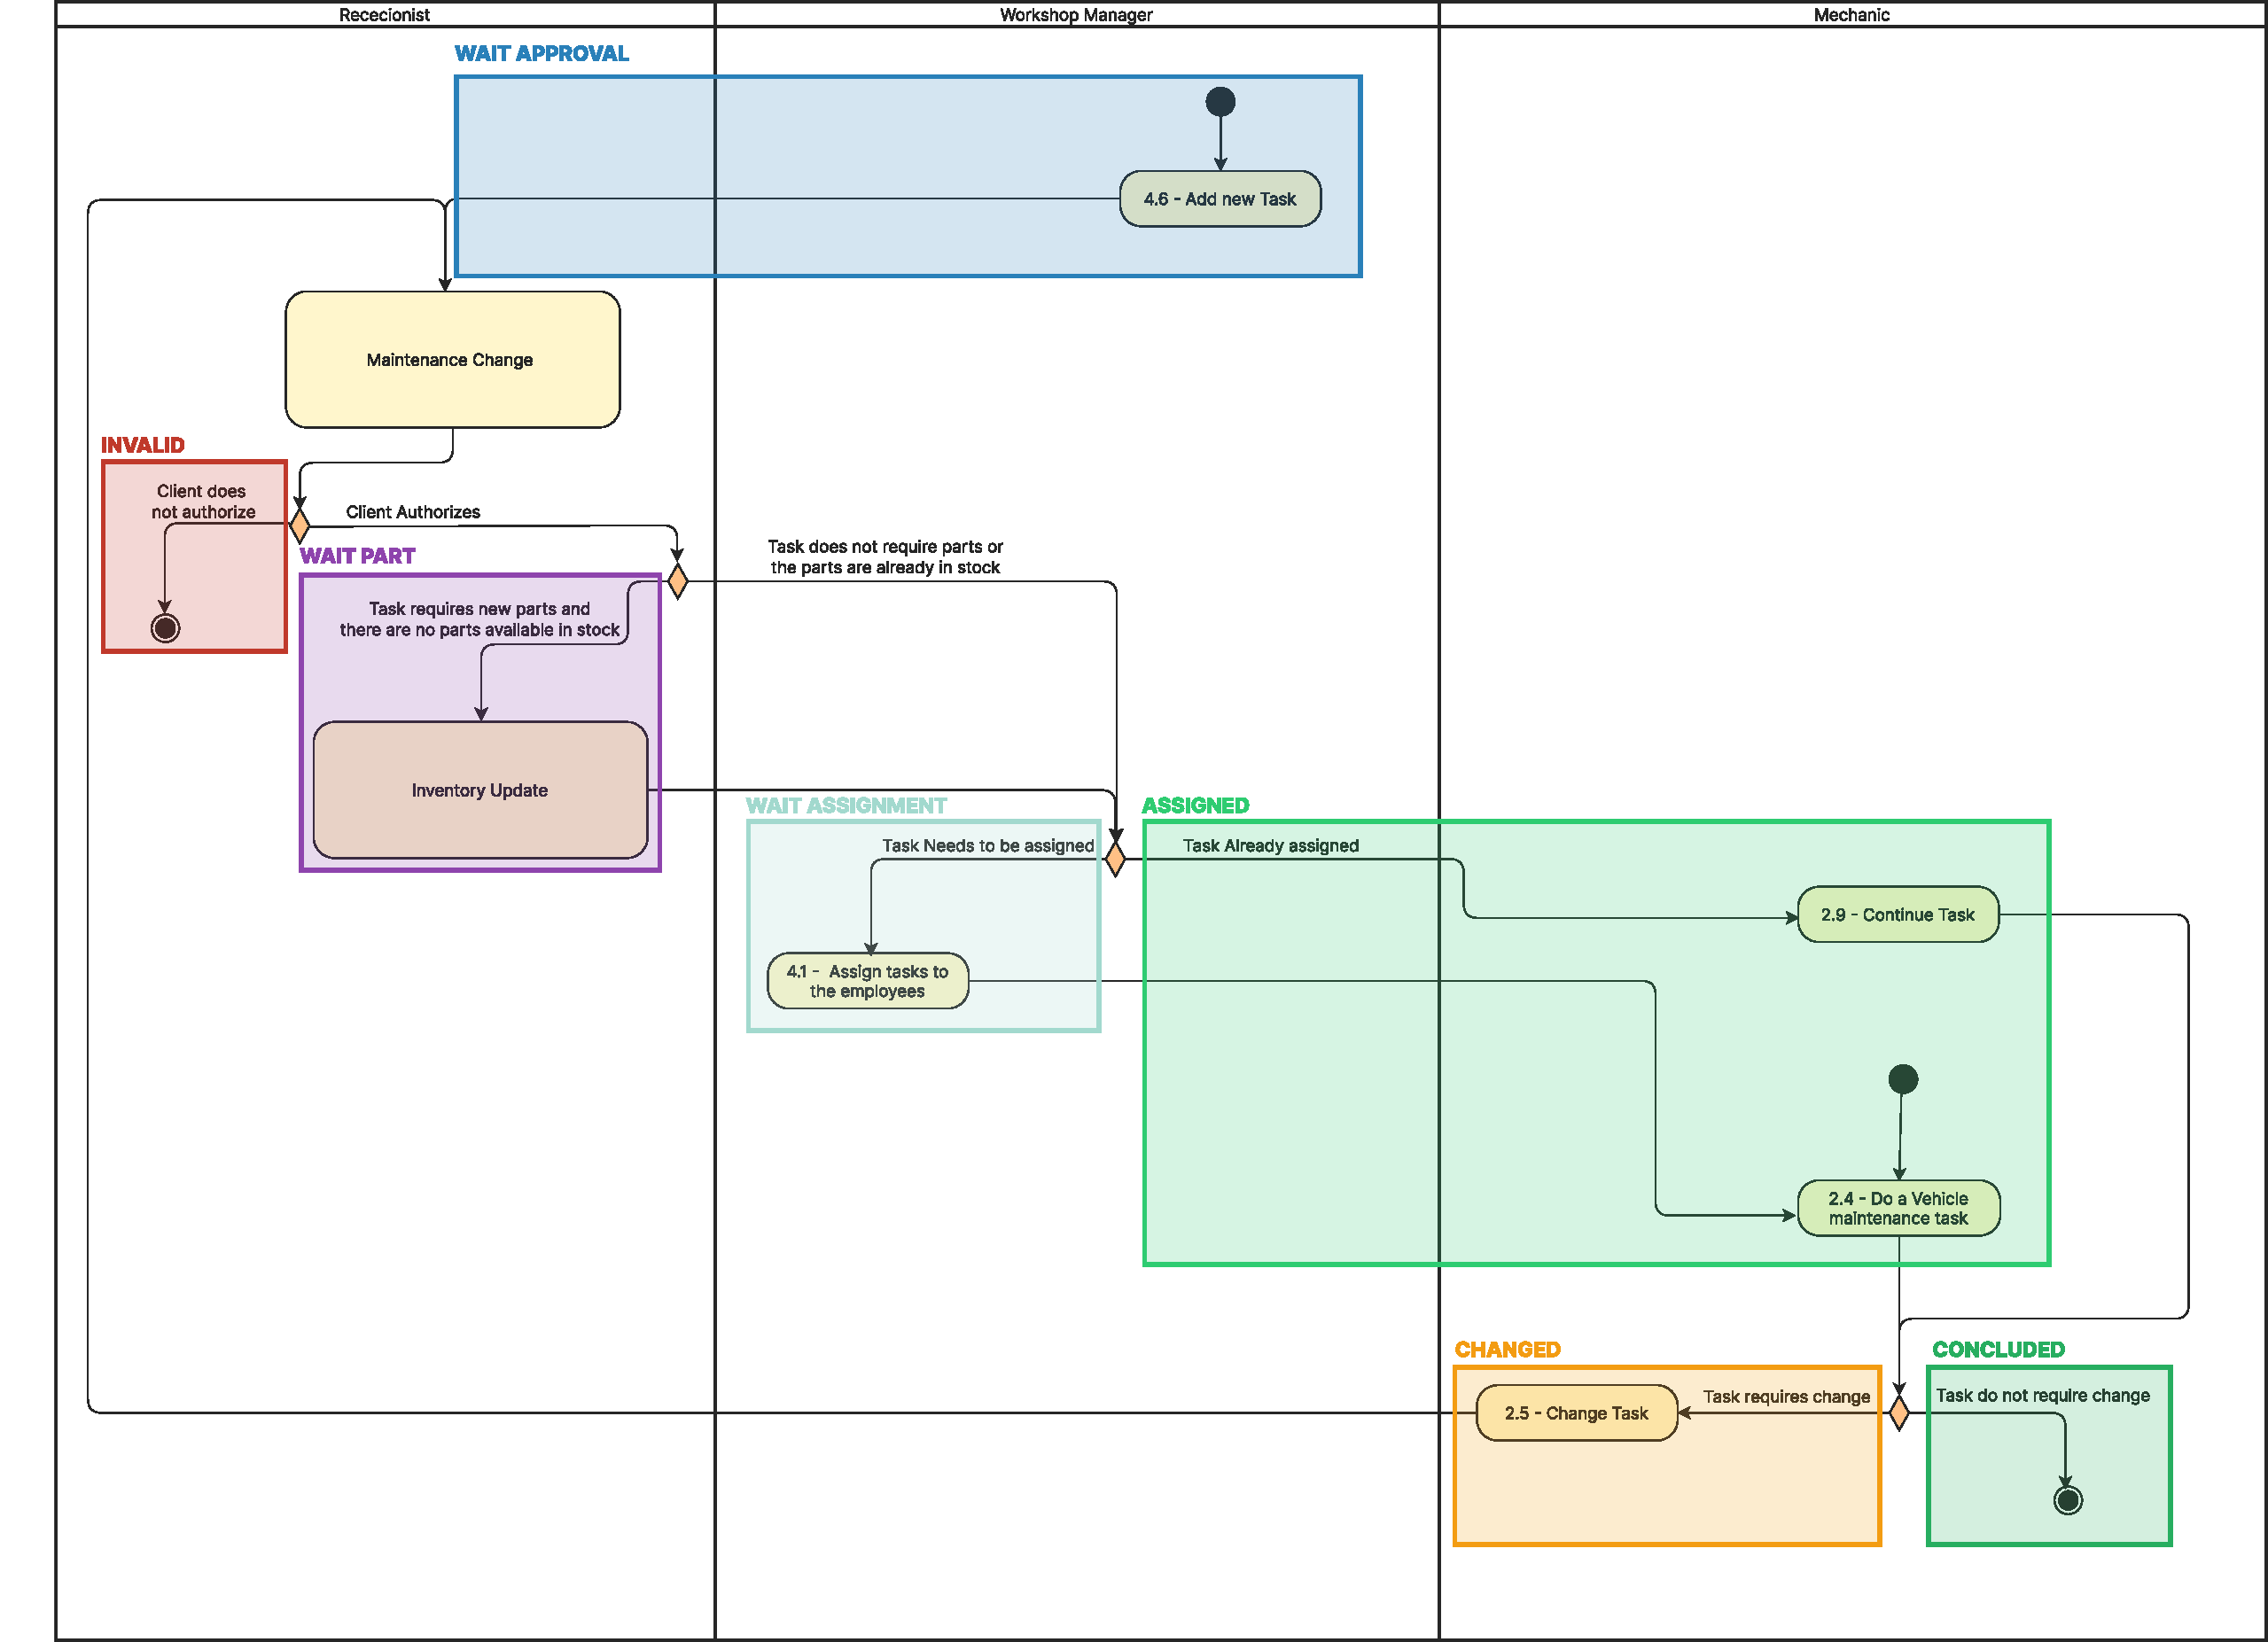
\includegraphics[width=\textwidth]{figs/Status/MaintenanceTask/UseCaseStatus}
  \label{fig:maintenanceTaskUseCase}
\end{figure}

\subsection{Purchase Status} 

In order to keep maintenance workflows uninterrupted, parts and materials often need to be acquired through a structured purchasing process. This process ensures that requests are validated, assigned, tracked, and properly registered once the items arrive. To guarantee accountability, the purchase workflow is modeled with a set of statuses that represent each step, from the initial request to its completion.

The \textit{purchase status} is defined by the following stages:
\begin{itemize}
\item \textbf{Wait Approval}: Initial status when a purchase request is submitted and awaits validation by the workshop manager.
\item \textbf{Invalid}: The request is rejected by the workshop manager and removed from the workflow.
\item \textbf{Assigned}: The request is approved and assigned to a warehouse operator.
\item \textbf{Wait Arrival}: The operator has contacted the supplier and is awaiting delivery of the requested parts.
\item \textbf{Finished}: The parts have arrived at the dealership and are registered into the system.
\end{itemize}

\begin{figure}[h]
  \caption{Status flow chart of a purchase}
  \centering
  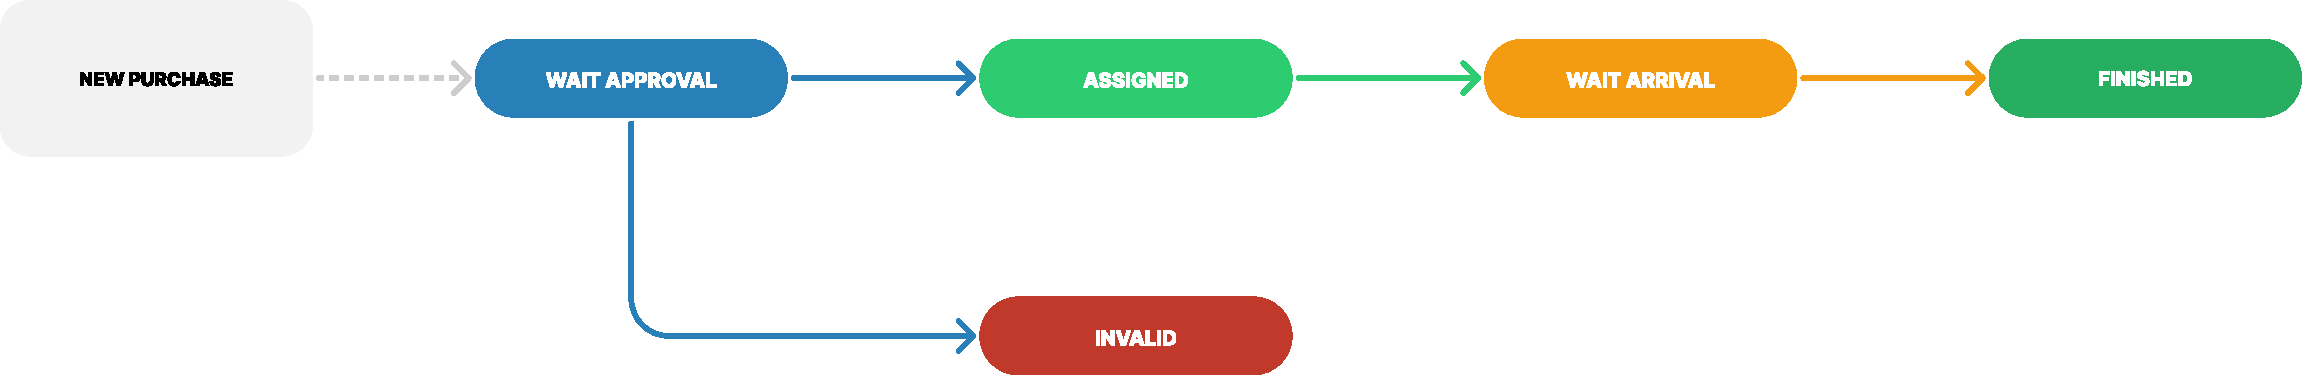
\includegraphics[width=\textwidth]{figs/Status/Purchase/StatusDiagram}
  \label{fig:purchaseFlowChart}
\end{figure}

The status transitions illustrated in Figure~\ref{fig:purchaseFlowChart} highlight the sequence of steps in a purchase workflow:
\begin{itemize}
\item \textbf{Wait Approval} $\rightarrow$ \textbf{Invalid}: If the workshop manager rejects the request.
\item \textbf{Wait Approval} $\rightarrow$ \textbf{Assigned}: If the request is approved.
\item \textbf{Assigned} $\rightarrow$ \textbf{Wait Arrival}: After the operator contacts the supplier and logs the expected delivery.
\item \textbf{Wait Arrival} $\rightarrow$ \textbf{Finished}: Once the parts arrive and are recorded in the system.
\end{itemize}


As shown in Figure~\ref{fig:purchaseUseCase}, the use case flow chart provides further detail by illustrating how purchase requests are initiated, validated, and completed. This structured process ensures that all acquisitions are traceable and properly integrated into the dealership's inventory.

\begin{figure}[h]
  \caption{Use case flow chart of a purchase, with statuses grouped by workflow steps}
  \centering
  \includegraphics[width=\textwidth]{figs/Status/Purchase/UseCaseStatus}
  \label{fig:purchaseUseCase}
\end{figure}


\subsection{Owner Partnership Status} 

To extend maintenance services beyond individual clients, dealerships may establish partnerships with organizations that own and manage vehicle fleets. The process is modeled through a simple status flow that tracks partnership requests and decisions.

The \textit{owner partnership status} consists of the following stages:

\begin{itemize}
\item \textbf{Request}: Initial state when a new entity submits a request to establish a partnership with the dealership.
\item \textbf{Accept}: The dealership approves the request, gaining access to the entity's vehicle information and authorization to schedule maintenance.
\item \textbf{Denied}: The dealership rejects the partnership request, ending the process.
\end{itemize}

\begin{figure}[h]
  \caption{Status flow chart of an owner partnership}
  \centering
  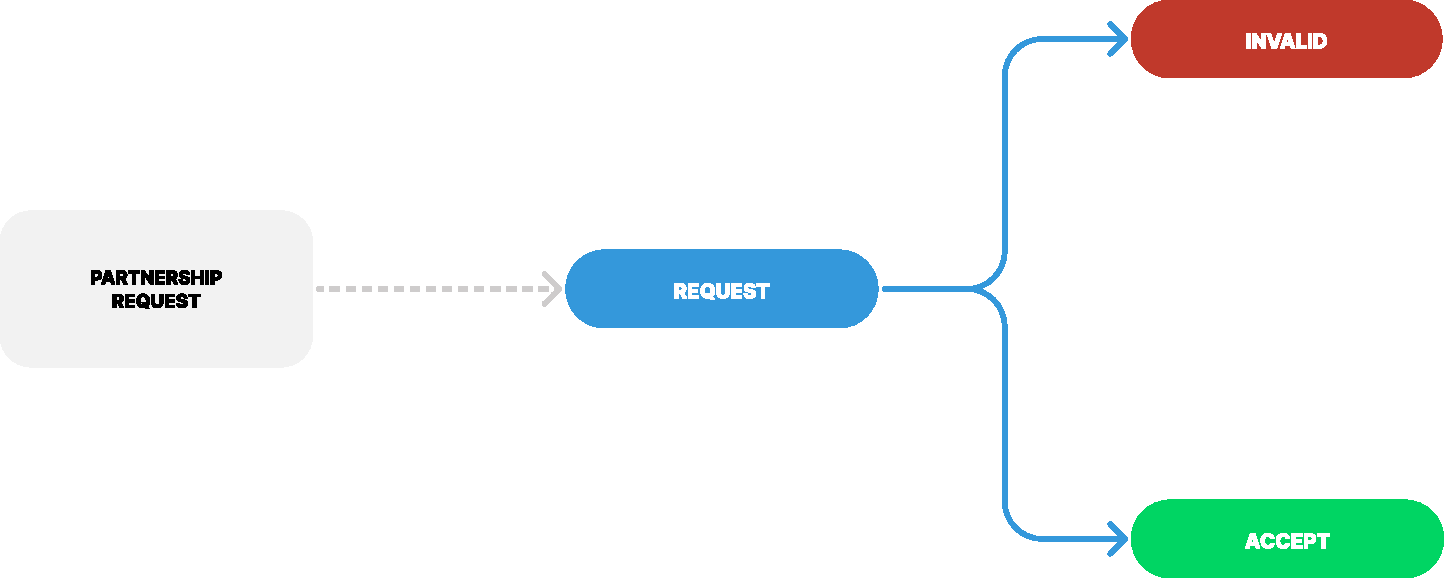
\includegraphics[width=\textwidth]{figs/Status/OwnerPartnership_StatusDiagram}
  \label{fig:ownerPartnershipFlowChart}
\end{figure}

This workflow, shown in Figure~\ref{fig:ownerPartnershipFlowChart}, ensures that all partnership requests are explicitly validated, preventing unauthorized access to sensitive vehicle data.





\section{Summary}


This chapter outlined the requirements analysis for the proposed maintenance management system, combining insights from stakeholder meetings and relevant literature. The requirements were structured using the FURPS model to address both functional and non-functional aspects of the system.

Functionally, the platform accommodates several user roles — including administrator, receptionist, mechanic, warehouse manager, workshop manager, and client — each responsible for specific tasks within the maintenance workflow. These range from managing data and inventory to scheduling services, executing maintenance operations, and providing client feedback.

The non-functional requirements defined key quality attributes such as scalability, reliability, performance, and usability, ensuring that the system remains robust, efficient, and compatible across major web browsers. The chapter also detailed the application’s workflow, describing how users interact throughout the maintenance process, from service scheduling to vehicle delivery, supported by clear communication and traceability mechanisms.

Finally, several operational status models were introduced to standardize and monitor system states — including maintenance, task, purchase, and partnership statuses — ensuring transparency and control across the maintenance lifecycle.

Altogether, this chapter established a solid foundation for the system’s design and implementation, ensuring that every requirement is well defined and aligned with stakeholder needs.